\documentclass{article}
\usepackage{a4wide}


\usepackage{polski}
\usepackage[utf8x]{inputenc}
\usepackage{graphicx}
\usepackage{float}
\usepackage{hyperref}
\usepackage{listings}
\usepackage{mathtools}
\usepackage{amsmath}
\usepackage{hyperref}
\usepackage[margin=1in]{geometry}

\author{Lev Sergeyev}
\title{ZAPDC \\ Ćwiczenie 4 \\ Algorytmy wygładzania I}

\date{ }
\begin{document}

\maketitle

%\pagebreakmovie15

\section{Przebieg ćwiczenia}
3 funkcję filtrujące:
\begin{itemize} 
	\item filtr splotowy, z paramertami:
	\begin{itemize} 
		\item kształt f-cji jądra (użyta funkcja Gaussa)
		\item długość f-cji jądra \(g_s \)
	\end{itemize}
	\item filtr medianowy
	\begin{itemize} 
		\item rozmiar okna
	\end{itemize}
	\item filtr bilateralny:
	\begin{itemize} 
		\item długość f-cji jądra (użyta funkcja Gaussa) \(g_s \)
		\item tolerancja różnic funkcji wygłądzającej (użyta funkcja Gaussa) \(f_s \)
	\end{itemize}
\end{itemize}

\section{Porównywanie filtrów}


\subsection{Filtr Splotowy}
\begin{center}
    \begin{tabular}{ | c | c | c |}
    \hline
    Parametry jądra & Błąd &  Obraz \\ \hline
    
    \smallskip kształt: funkcja Gaussa, \(g_s = 3\) & 37.57 &
    \raisebox{-\totalheight}{\scalebox{0.2}{
\includegraphics{img/s5.png}}}
    
     \\ \hline
	
    \smallskip kształt: funkcja Gaussa,\(g_s = 4\) & 35.82 &
    \raisebox{-\totalheight}{\scalebox{0.2}{
\includegraphics{img/s7.png}}} 
    
    \\ \hline
    \end{tabular}
\end{center}


\subsection{Filtr Medianowy}
\begin{center}
    \begin{tabular}{ | c | c | c |}
    \hline
    Rozmiar okna & Błąd &  Obraz \\ \hline
    
    5x5 & 37.06 &
    \raisebox{-\totalheight}{\scalebox{0.2}{
\includegraphics{img/m5.png}}}
    
     \\ \hline
	
    7x7 & 34.43 &
    \raisebox{-\totalheight}{\scalebox{0.2}{
\includegraphics{img/m7.png}}} 
    
    \\ \hline
    \end{tabular}
\end{center}

\subsection{Filtr Bilateralny}
\begin{center}
    \begin{tabular}{ | c | c | c |}
    \hline
    Parametry jądra & Błąd &  Obraz \\ \hline
    
    \smallskip kształt: funkcja Gaussa, \( f_r = 50, g_s = 3\) & 40.65 &
    \raisebox{-\totalheight}{\scalebox{0.2}{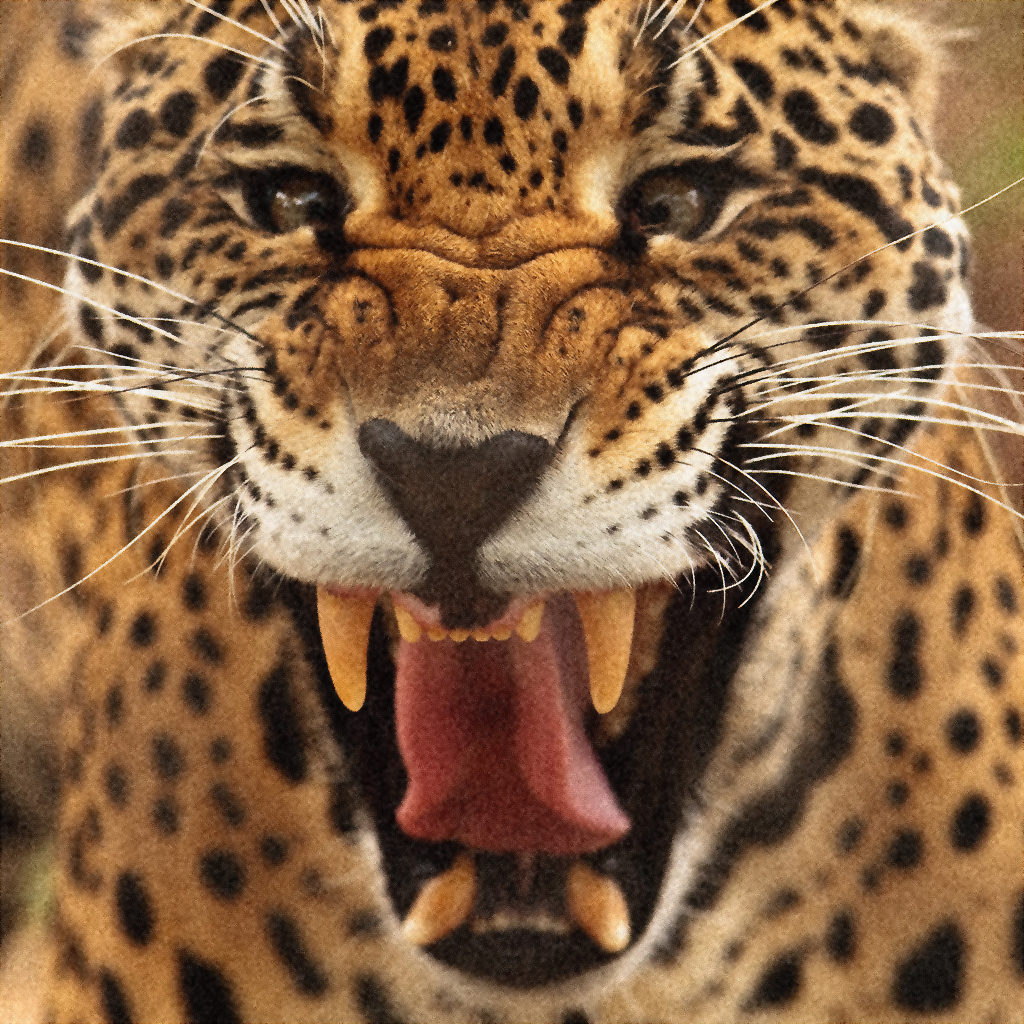
\includegraphics{img/b5.png}}}
    
     \\ \hline
	
    \smallskip kształt: funkcja Gaussa, \( f_r = 50, g_s = 4\) & 38.95 &
    \raisebox{-\totalheight}{\scalebox{0.2}{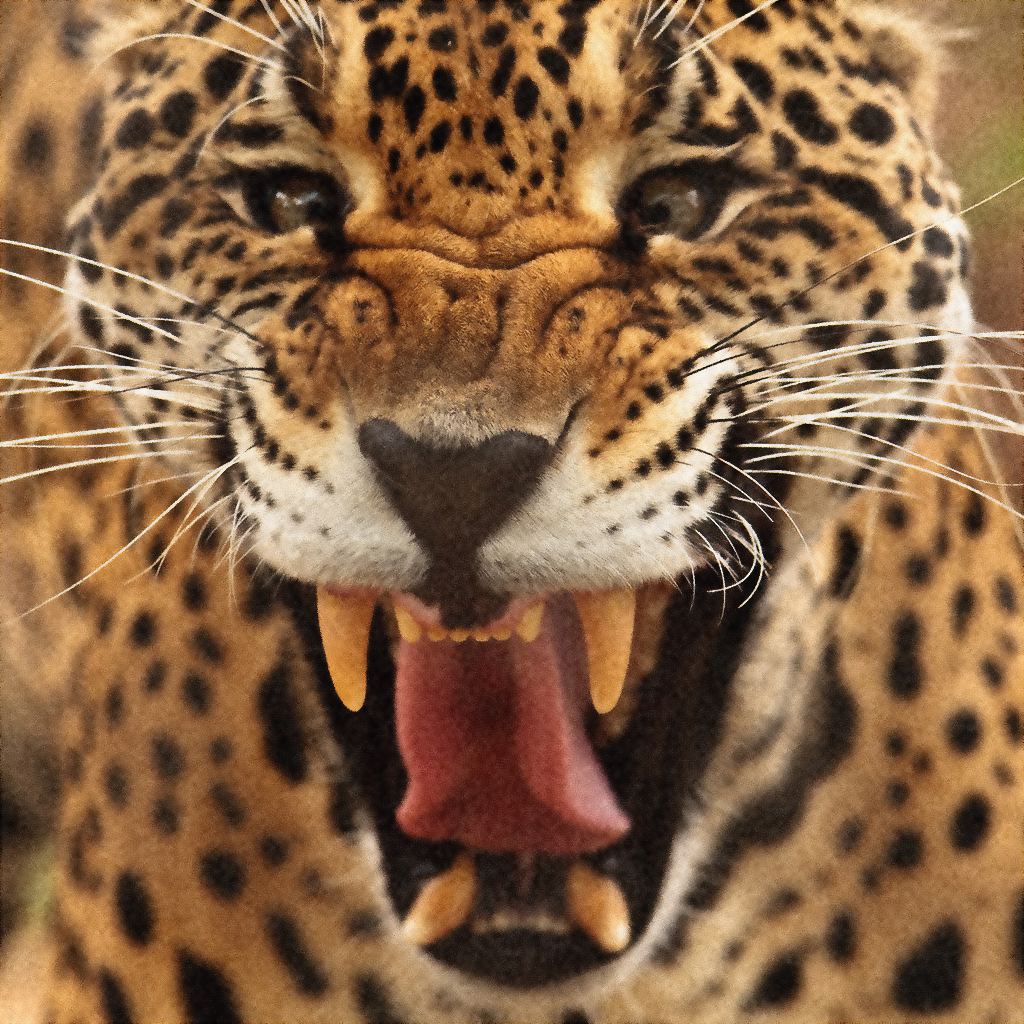
\includegraphics{img/b7.png}}} 
    
    \\ \hline
    \end{tabular}
\end{center}

\pagebreak


\subsection{Kod}
\href{https://github.com/221349/ZAPDC/tree/master/lab7}{https://github.com/221349/ZAPDC/tree/master/lab7}

\section{Wnioski}
\par
Porównując wyniki działań filtrów, można stwierdzić, że zachować jaknajwięcej szczegółów a przy tym przeprowadzić jaknajwiększe odszumianie może filtr bilateralny. \\

Odszumić i zachować jaknajwiększe podobieństwo liczbow do obrazu oryginalnego może filtr medianowy. Przydatny jest kiedy potrzebujemy dokładnie zachować kształty i granice.
\\

Filtr splotowy przydatny jest w przypadku odszumiania gradientów i płynnych przejść.




\end{document}
